%!TEX TS-program = xelatex
%!TEX encoding = UTF-8 Unicode

\documentclass[a4paper,openany,12pt]{ctexbook}
\def\mathfamilydefault{\rmdefault}

\setlength\paperheight{29.7cm}%高度
\setlength\paperwidth{21cm}%宽度
\XeTeXlinebreaklocale “zh”
\XeTeXlinebreakskip = 0pt plus 1pt minus 0.1pt %文章内中文自动换行

%\usepackage{ctex}
\usepackage{fontspec,xltxtra,xunicode}
% \usepackage[slantfont,boldfont,CJKnumber,CJKtextspaces]{xeCJK}% 调用 xeCJK 宏包
\usepackage{xeCJK}
\usepackage{pdfpages}%插入封面pdf文件
\usepackage{geometry}   %设置页边距的宏包, 定制页面格式
\usepackage{titlesec}   %设置页眉页脚的宏包
% \usepackage{makeidx}
\usepackage{fancyhdr}% 设置页眉页脚
\usepackage{indentfirst}%第一段首行缩进
% 其它需要使用的宏包
% \usepackage[colorlinks,linkcolor=blue,anchorcolor=red,citecolor=green,urlcolor=blue]{hyperref}  
\usepackage{tabularx}
% \usepackage{abstract}
\usepackage{authblk}% 作者信息
% \usepackage{algorithm}% 算法排版
\usepackage{amsmath}% 数学符号与式
\usepackage{amsfonts}% 数学符号与字体
\usepackage{graphics}
\usepackage{caption}
\usepackage{color}
\usepackage{fancyvrb}% 抄录环境
\usepackage{float}% 管理浮动体
\usepackage{hyperref}% 为PDF文档创建超链接
\usepackage{lineno}% 生成行号
\usepackage{listings}% 插入程序源代码
\usepackage{multicol} % 多栏排版
\usepackage{natbib} % 管理文献引用
\usepackage[figuresright]{rotating}% 旋转文字,图形,表格
\usepackage{subfig}% 排版子图形
\usepackage{moresize} % 更多字体大小
\usepackage{anysize}
\usepackage{booktabs} % 使用\multicolumn
\usepackage{multirow} % 使用\multirow
\usepackage{graphicx}  
\usepackage{wrapfig}
\usepackage{xcolor}
\usepackage{enumitem}
\usepackage{hyperref}
\usepackage{setspace} 
\usepackage{booktabs}
\usepackage{float,subfloat}
\usepackage{amsmath}
% \usepackage{enumerate}

%%%%%%%%%%%%%%%%%%%%%%%%%%%%%%%%%%%%%%%%%%新加的
\usepackage{bm}
\usepackage{multirow, amsthm, amssymb,graphicx,dashbox}
\usepackage{lscape}
\usepackage[ruled]{algorithm2e}
\modulolinenumbers[5]
\newtheorem{theorem}{\songticu 定理}[section]
%\newtheorem{proof}{证明}[section]
%\newtheorem{lemma}{\hspace{2em}引理}[chapter]
\newtheorem{remark}{\songticu 评论}[section]

\usepackage{colortbl}
\usepackage{arydshln}
\usepackage{multirow}
\usepackage{multicol}

\usepackage{dsfont}
\hypersetup{hidelinks}
\usepackage{setspace}

\usepackage{titletoc}
\titlecontents{chapter}[0pt]{\normalfont\HEITI\addvspace{2pt}\filright}  %章节标题在目录中也有虚线            
{\contentspush{\thecontentslabel\ }}              
{}{\titlerule*[8pt]{.}\contentspage}

\usepackage{setspace} 
%\usepackage{mathrsfs}%花体字母
%\usepackage{stmaryrd}%空心中括号
%%%%%%%%%%%%%%%%%%%%%%%%%%%%%%%%%%%%%%%%%%

\setCJKfamilyfont{songsong}{SimSun}
\newcommand*{\SONGTI}{\CJKfamily{songsong}} 
\setCJKfamilyfont{heihei}{SimHei}
\newcommand*{\HEITI}{\CJKfamily{heihei}} 
\setCJKfamilyfont{songticu}[Path=Fonts/]{stsongti-sc-bold.ttf}
\newcommand*{\songticu}{\CJKfamily{songticu}} 

\setCJKmainfont{SimSun}% 设置 CJK 主字体为宋体
\setmainfont{Times New Roman}
\graphicspath{{figures/}} %安放图片路径

\geometry{left=2.5cm,right=2.5cm,top=2.5cm,bottom=3cm}%在有页眉上页边距2.1cm,下、左、右页边距都是2.5cm;
\defaultfontfeatures{Mapping=tex-text} %如果没有它,会有一些 tex 特殊字符无法正常使用,比如连字符。
%\renewcommand{\baselinestretch}{2.5}%1.5倍行距。
\linespread{1.68}\selectfont%经过多次尝试与word1.5倍行距最为接近
\parskip=0pt %段间距离同行距
%\renewcommand{\algorithmicrequire}{ \textbf{Input:}} %Use Input in the format of Algorithm  
%\renewcommand{\algorithmicensure}{ \textbf{Output:}} %UseOutput in the format of Algorithm  
% 中文就是要放在中文环境里,使用如下
\renewcommand{\algorithmcfname}{\songticu 算法}


\newcommand{\chuhao}{\fontsize{42pt}{\baselineskip}\selectfont}
\newcommand{\xiaochuhao}{\fontsize{36pt}{\baselineskip}\selectfont}
\newcommand{\yihao}{\fontsize{28pt}{\baselineskip}\selectfont}
\newcommand{\erhao}{\fontsize{21pt}{\baselineskip}\selectfont}
\newcommand{\xiaoerhao}{\fontsize{18pt}{\baselineskip}\selectfont}
\newcommand{\sanhao}{\fontsize{15.75pt}{\baselineskip}\selectfont}
\newcommand{\sihao}{\fontsize{14pt}{\baselineskip}\selectfont}
\newcommand{\xiaosihao}{\fontsize{12pt}{\baselineskip}\selectfont}
\newcommand{\wuhao}{\fontsize{10.5pt}{\baselineskip}\selectfont}
\newcommand{\xiaowuhao}{\fontsize{9pt}{\baselineskip}\selectfont}
\newcommand{\liuhao}{\fontsize{7.875pt}{\baselineskip}\selectfont}
\newcommand{\qihao}{\fontsize{5.25pt}{\baselineskip}\selectfont}

\renewcommand\floatpagefraction{.9}
\renewcommand\topfraction{.9}
\renewcommand\bottomfraction{.9}
\renewcommand\textfraction{.1}
\setcounter{totalnumber}{50}
\setcounter{topnumber}{50}
\setcounter{bottomnumber}{50}

% 将默认的英文目录等改为中文,设置图号和式号与章节对应,缩进大小
% % \titleformat{命令}[形式]{<b>格式</b>}{标题头定义}{间距}{前命令}[后命令]
%==================================================
\titleformat{\title}[display]{\normalfont\erhao\centering}{}{0.2cm}{}[\vspace{-1cm}] %题目: 二号宋体居中
\titleformat{\chapter}[hang]{\normalfont\sanhao\centering\HEITI}{第{\chinese{chapter}}章}{0.2cm}{}%[\vspace{-1cm}] %章:三号黑体并居中
\titleformat{\section}[hang]{\normalfont\sihao\bfseries\songticu}{\thesection}{0.2cm}{} %节:四号宋体(粗体)居左
\titleformat{\subsection}[hang]{\normalfont\xiaosihao}{\thesubsection}{0.2cm}{} %节内小节:小四宋体居左
\titleformat{\subsubsection}[hang]{\normalfont\xiaosihao}{\thesubsubsection}{0.2cm}{} %子目:小四宋体居左

\titlespacing*{\chapter} {0pt}{-20pt}{20pt}%__上下

\DeclareCaptionFont{capFont}{\normalfont\wuhao} % 表格名及图名用5号宋体
\DeclareCaptionLabelSeparator{twospace}{~~}
\captionsetup{
	labelsep=twospace,% 去掉图标签后的冒号
	font={capFont},%
	figurename=图,%
	tablename=表%
	% listfigurename=插图目录,%
	% listtablename=表格目录}
}
\makeatother
%==================================================

\title{南京信息工程大学硕士毕业论文模板}%大论文题目

\begin{document}
\newcommand{\upcite}[1]{\textsuperscript{\textsuperscript{\cite{#1}}}}
	\xiaosihao%内芯用小四号字
%	\includepdf[pages=1-4]{coverfinal2.pdf}%插入多页封面
	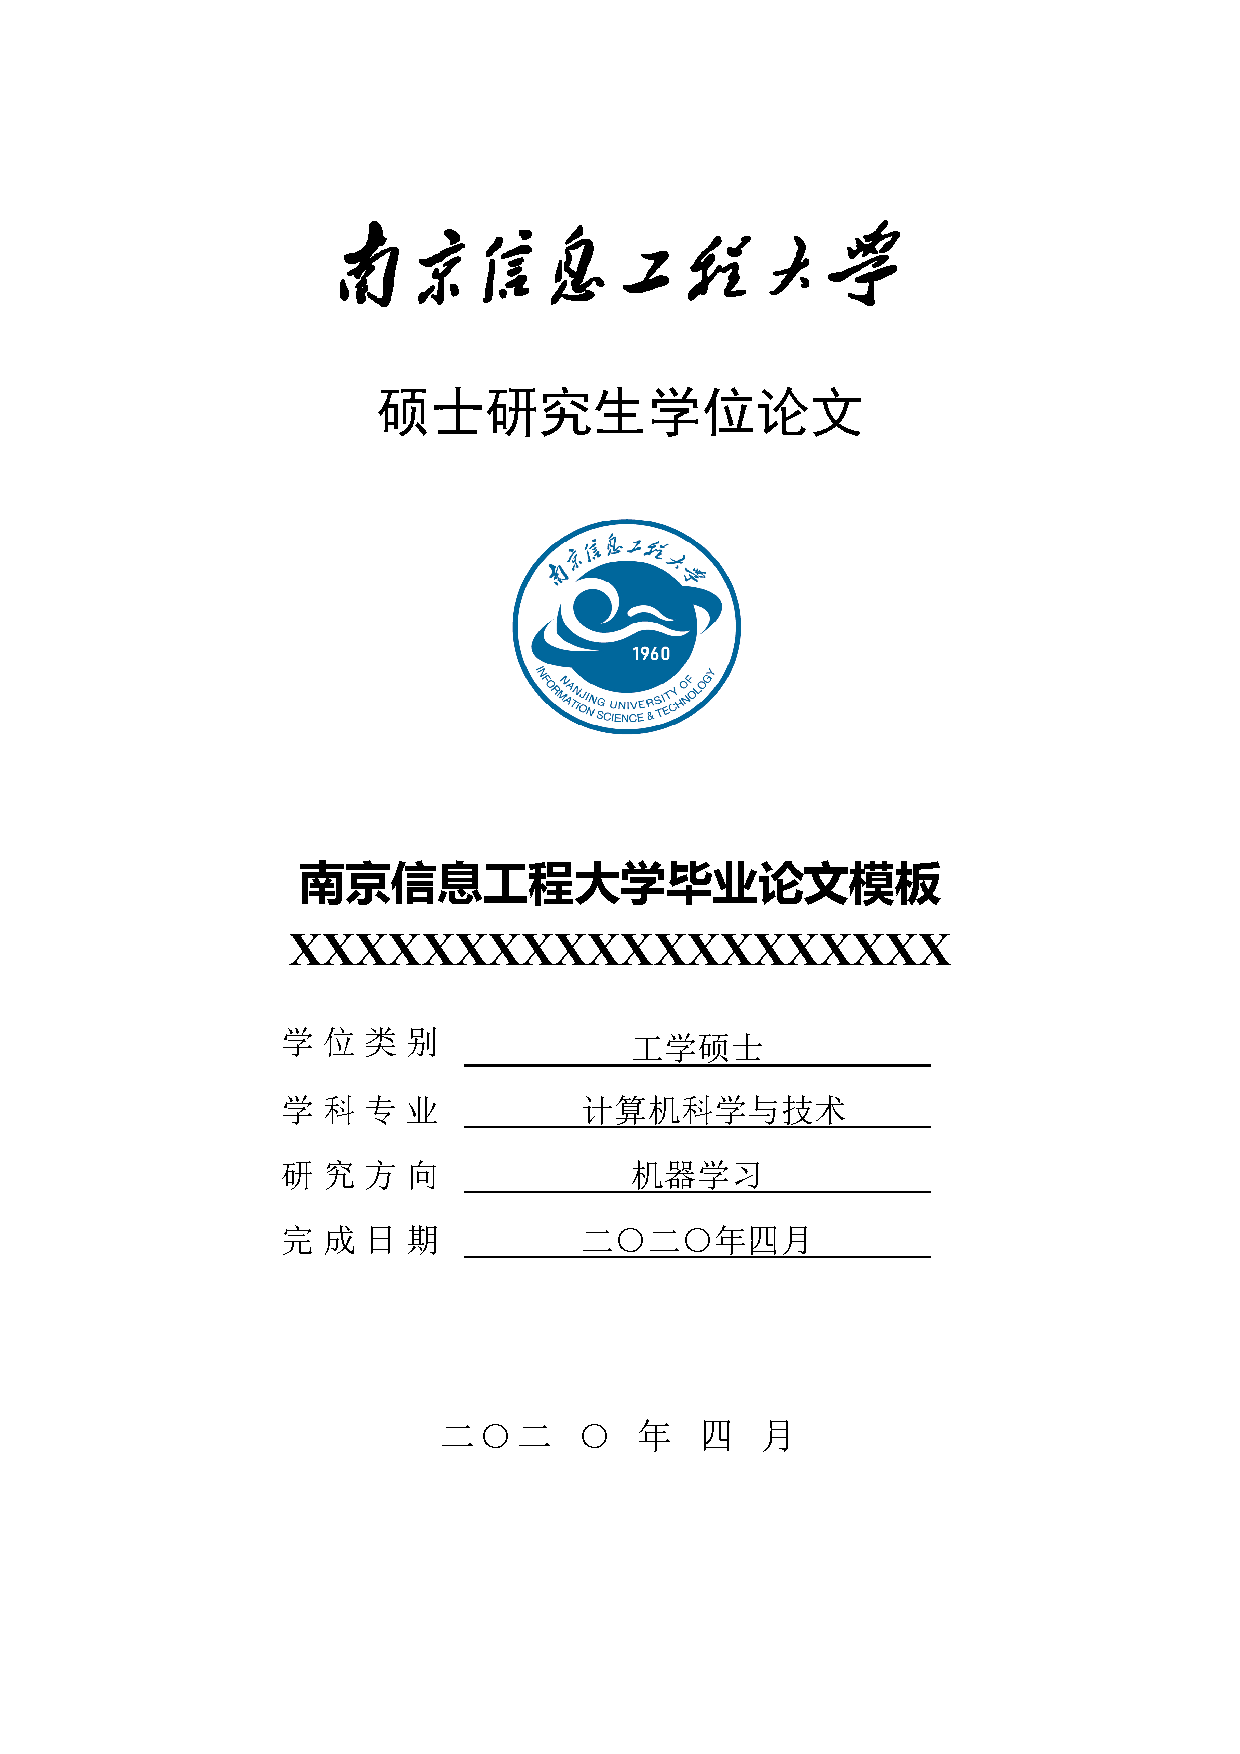
\includepdf{coverblind1.pdf} %插入盲审封面
	
\includepdf{coverblind2.pdf} %插入承诺书
	
	\newgeometry{left=2.5cm,right=2.5cm,top=2.5cm,bottom=3cm}%无页眉上下左右页边距都是2.5cm。
	\pagenumbering{Roman}%% 前面摘要和目录等内容的页码用大写罗马数字表示。
	\pagestyle{plain}%只有页码
	\begin{spacing}{1.43}
		\tableofcontents %插入目录
	\end{spacing}
	\newpage
	\pagenumbering{Roman}%% 摘要重新开始编页,前面摘要和目录等内容的页码用大写罗马数字表示。
	\begin{spacing}{0.8}
	\chapter*{摘\quad 要} 
	\end{spacing}
	\begin{spacing}{1.63}
	\addcontentsline{toc}{chapter}{摘\quad 要}
	此模板为南信大硕士毕业论文模板,由单滢滢、耿祥编写,由耿祥整理发布。模板Github主页为\url{https://github.com/hy5468/NUIST-LaTeX},请大家给该项目打星。
	\\
	\end{spacing}	
	\begin{spacing}{1.63}
		\noindent{\songticu 关键词:} 
	\end{spacing}		
	\begin{spacing}{1.0}
	\chapter*{Abstract} 
	\end{spacing}
	\addcontentsline{toc}{chapter}{Abstract}
	此模板为南信大硕士毕业论文模板,由单滢滢、耿祥编写,由耿祥整理发布。模板Github主页为\url{URL},请大家给该项目打星(假装自己是英文)。
	\\
	\noindent\textbf{Keywords: } 


	%%%%%%%%%%%%%%%%%%%%%%%%%%%%%%%%%%%%%%%%%	
	\newpage
	\mainmatter %% 论文页码1从正文开始
	%\author{耿祥}%作者信息
	\newpage
	\restoregeometry %重置页边距
	\pagestyle{fancy}%设置页眉
	\fancyhf{}
	\fancyhead[CO]{\zihao{-5}\leftmark}
	\fancyhead[CE]{\zihao{-5} 南京信息工程大学硕士学位论文}
	\fancyfoot[C]{\thepage} 
	\fancypagestyle{plain}{
		\pagestyle{fancy}
	}
	\chapter{模板使用}\def\leftmark{第一章\quad 模板使用} 
\begin{spacing}{1.4}
	\section{标题}
\end{spacing}
	\cite{lecun2015deep}引用示例,上标引用示例\upcite{lecun2015deep}。
	\begin{eqnarray}
	E=mc^2
	\end{eqnarray}
	\begin{theorem}\label{theorem1}
		定理样例。
	\end{theorem}
	\renewcommand*{\qedsymbol}{[\songticu{证毕}]}
	\begin{proof}[{\songticu 证定理 \ref{theorem1} :}]
		因为所以自然有理。
	\end{proof}
	\subsection{标题}
	\begin{figure}[!htbp]
		\centering
		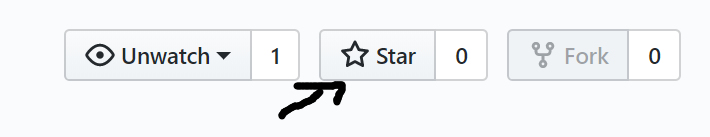
\includegraphics[scale=0.5]{./fig/1.png}
		\caption{图片示例}
		\label{fig1}
	\end{figure}
	
	\begin{itemize}[leftmargin=0.2in]
		\setlength{\itemsep}{-1pt}
		\item \emph{方法1:}
		
		\item \emph{方法2:} 

		\item \emph{方法3:} 
	\end{itemize}
	
	
\begin{table*}[t]
	\centering
	\caption{表格示例}
	\label{tab:dataset}
	\linespread{1.5}\selectfont
	\begin{tabular}{ccccc}
		\toprule
		\multicolumn{5}{c}{数据}\\
		\midrule
		名称		&训练样本	     &总样本  & 特征数  & 类别数 \\
		\midrule
		
		 &	& 		&	    & \\
		 &	& 		&	    & \\
		 &	& 		&	    & \\
		 &	& 		&	    & \\
		\midrule
		\multicolumn{5}{c}{数据}\\
		\midrule
		名称		&训练样本	     &总样本  & 特征数  & 类别数 \\
		\midrule
		&	& 		&	    & \\
		&	& 		&	    & \\
		&	& 		&	    & \\
		&	& 		&	    & \\
		\bottomrule
	\end{tabular}
\end{table*}

\begin{figure*}[htb]
	\centering
\subfloat[A]{
	\begin{minipage}[b]{0.46\textwidth}
		\centering
		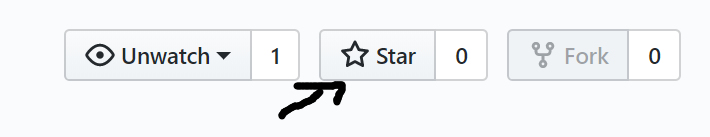
\includegraphics[width=2.1in]{./fig/1.png}
	\end{minipage}
}
	\subfloat[B]{
	\begin{minipage}[b]{0.46\textwidth}
		\centering
		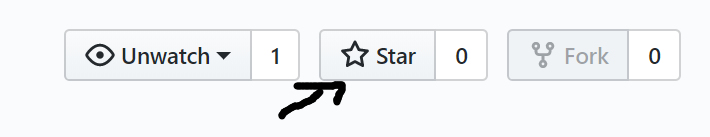
\includegraphics[width=2.1in]{./fig/1.png}
	\end{minipage}
}\\
	\subfloat[C]{
	\begin{minipage}[b]{0.46\textwidth}
		\centering
		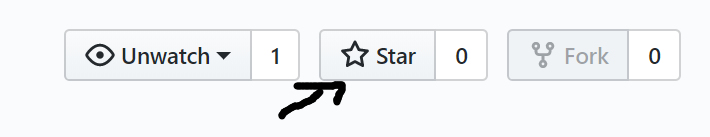
\includegraphics[width=2.1in]{./fig/1.png}
	\end{minipage}
}
	\subfloat[D]{
	\begin{minipage}[b]{0.46\textwidth}
		\centering
		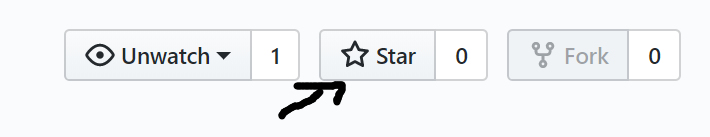
\includegraphics[width=2.1in]{./fig/1.png}
	\end{minipage}
}\\
	\subfloat[E]{
	\begin{minipage}[b]{0.46\textwidth}
		\centering
		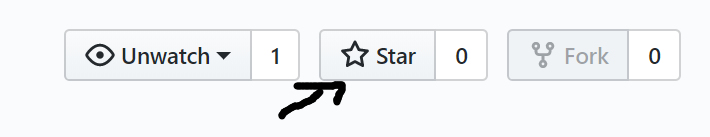
\includegraphics[width=2.1in]{./fig/1.png}
	\end{minipage}
}
	\subfloat[F]{
	\begin{minipage}[b]{0.46\textwidth}
		\centering
		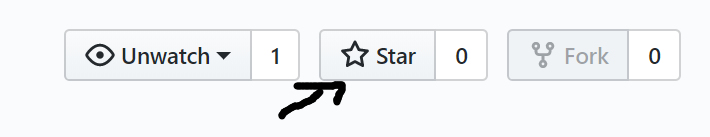
\includegraphics[width=2.1in]{./fig/1.png}
	\end{minipage}
}\\
	\subfloat[G]{
	\begin{minipage}[b]{0.46\textwidth}
		\centering
		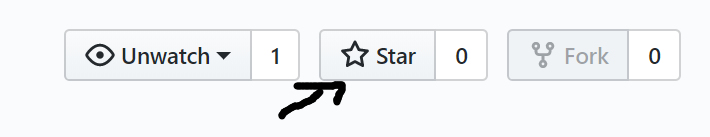
\includegraphics[width=2.1in]{./fig/1.png}
	\end{minipage}
}
	\subfloat[H]{
	\begin{minipage}[b]{0.46\textwidth}
		\centering
		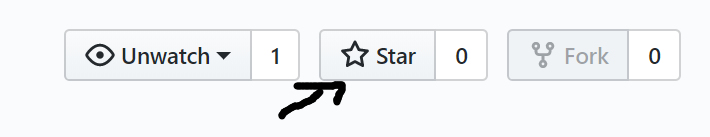
\includegraphics[width=2.1in]{./fig/1.png}
	\end{minipage}
}
	\caption{
		多图示例
	}
	\label{fig2}
\end{figure*}

\def\leftmark{参考文献} 
\begin{thebibliography}{70}
	\addtolength{\itemsep}{-1em}
	\bibliographystyle{unsrt}	
	
	\bibitem[LeCun et~al.(2015)LeCun, Bengio, and Hinton]{lecun2015deep}
	LeCun, Y., Bengio, Y., and Hinton, G.
	\newblock Deep learning.
	\newblock \emph{nature}, 521\penalty0 (7553):\penalty0 436--444, 2015.	
\end{thebibliography}
\addcontentsline{toc}{chapter}{参考文献}
\chapter*{致\quad 谢} \def\leftmark{致\quad 谢} 
\addcontentsline{toc}{chapter}{致\quad 谢}


\chapter*{作者简介}\def\leftmark{作者简介} 
\addcontentsline{toc}{chapter}{作者简介}
\section*{{\songticu 基本情况:}}


\section*{{\songticu 硕士期间完成的学术论文:}}


\end{document}